% Options for packages loaded elsewhere
\PassOptionsToPackage{unicode}{hyperref}
\PassOptionsToPackage{hyphens}{url}
%
\documentclass[
  english,
  man,floatsintext]{apa6}
\usepackage{lmodern}
\usepackage{amssymb,amsmath}
\usepackage{ifxetex,ifluatex}
\ifnum 0\ifxetex 1\fi\ifluatex 1\fi=0 % if pdftex
  \usepackage[T1]{fontenc}
  \usepackage[utf8]{inputenc}
  \usepackage{textcomp} % provide euro and other symbols
\else % if luatex or xetex
  \usepackage{unicode-math}
  \defaultfontfeatures{Scale=MatchLowercase}
  \defaultfontfeatures[\rmfamily]{Ligatures=TeX,Scale=1}
\fi
% Use upquote if available, for straight quotes in verbatim environments
\IfFileExists{upquote.sty}{\usepackage{upquote}}{}
\IfFileExists{microtype.sty}{% use microtype if available
  \usepackage[]{microtype}
  \UseMicrotypeSet[protrusion]{basicmath} % disable protrusion for tt fonts
}{}
\makeatletter
\@ifundefined{KOMAClassName}{% if non-KOMA class
  \IfFileExists{parskip.sty}{%
    \usepackage{parskip}
  }{% else
    \setlength{\parindent}{0pt}
    \setlength{\parskip}{6pt plus 2pt minus 1pt}}
}{% if KOMA class
  \KOMAoptions{parskip=half}}
\makeatother
\usepackage{xcolor}
\IfFileExists{xurl.sty}{\usepackage{xurl}}{} % add URL line breaks if available
\IfFileExists{bookmark.sty}{\usepackage{bookmark}}{\usepackage{hyperref}}
\hypersetup{
  pdftitle={Re-analysing the data from Moffatt et al. (2020): A textbook illustration of the fallacy of the null hypothesis},
  pdflang={en-EN},
  pdfkeywords={NHST, Bayesian, fallacy, reanalysis, inner speech, rumination, electromyography},
  hidelinks,
  pdfcreator={LaTeX via pandoc}}
\urlstyle{same} % disable monospaced font for URLs
\usepackage{graphicx}
\makeatletter
\def\maxwidth{\ifdim\Gin@nat@width>\linewidth\linewidth\else\Gin@nat@width\fi}
\def\maxheight{\ifdim\Gin@nat@height>\textheight\textheight\else\Gin@nat@height\fi}
\makeatother
% Scale images if necessary, so that they will not overflow the page
% margins by default, and it is still possible to overwrite the defaults
% using explicit options in \includegraphics[width, height, ...]{}
\setkeys{Gin}{width=\maxwidth,height=\maxheight,keepaspectratio}
% Set default figure placement to htbp
\makeatletter
\def\fps@figure{htbp}
\makeatother
\setlength{\emergencystretch}{3em} % prevent overfull lines
\providecommand{\tightlist}{%
  \setlength{\itemsep}{0pt}\setlength{\parskip}{0pt}}
\setcounter{secnumdepth}{-\maxdimen} % remove section numbering
% Make \paragraph and \subparagraph free-standing
\ifx\paragraph\undefined\else
  \let\oldparagraph\paragraph
  \renewcommand{\paragraph}[1]{\oldparagraph{#1}\mbox{}}
\fi
\ifx\subparagraph\undefined\else
  \let\oldsubparagraph\subparagraph
  \renewcommand{\subparagraph}[1]{\oldsubparagraph{#1}\mbox{}}
\fi
% Manuscript styling
\usepackage{upgreek}
\captionsetup{font=singlespacing,justification=justified}

% Table formatting
\usepackage{longtable}
\usepackage{lscape}
% \usepackage[counterclockwise]{rotating}   % Landscape page setup for large tables
\usepackage{multirow}		% Table styling
\usepackage{tabularx}		% Control Column width
\usepackage[flushleft]{threeparttable}	% Allows for three part tables with a specified notes section
\usepackage{threeparttablex}            % Lets threeparttable work with longtable

% Create new environments so endfloat can handle them
% \newenvironment{ltable}
%   {\begin{landscape}\begin{center}\begin{threeparttable}}
%   {\end{threeparttable}\end{center}\end{landscape}}
\newenvironment{lltable}{\begin{landscape}\begin{center}\begin{ThreePartTable}}{\end{ThreePartTable}\end{center}\end{landscape}}

% Enables adjusting longtable caption width to table width
% Solution found at http://golatex.de/longtable-mit-caption-so-breit-wie-die-tabelle-t15767.html
\makeatletter
\newcommand\LastLTentrywidth{1em}
\newlength\longtablewidth
\setlength{\longtablewidth}{1in}
\newcommand{\getlongtablewidth}{\begingroup \ifcsname LT@\roman{LT@tables}\endcsname \global\longtablewidth=0pt \renewcommand{\LT@entry}[2]{\global\advance\longtablewidth by ##2\relax\gdef\LastLTentrywidth{##2}}\@nameuse{LT@\roman{LT@tables}} \fi \endgroup}

% \setlength{\parindent}{0.5in}
% \setlength{\parskip}{0pt plus 0pt minus 0pt}

% \usepackage{etoolbox}
\makeatletter
\patchcmd{\HyOrg@maketitle}
  {\section{\normalfont\normalsize\abstractname}}
  {\section*{\normalfont\normalsize\abstractname}}
  {}{\typeout{Failed to patch abstract.}}
\makeatother
\shorttitle{The fallacy of the null}
\author{Ladislas Nalborczyk\textsuperscript{1}}
\affiliation{
\vspace{0.5cm}
\textsuperscript{1} Univ. Grenoble Alpes, CNRS, Grenoble INP, GIPSA-lab, 38000 Grenoble, France}
\authornote{

Correspondence concerning this article should be addressed to Ladislas Nalborczyk, GIPSA-lab, CNRS, Univ. Grenoble Alpes, 11 Rue des Mathématiques, 38400 Saint-Martin-d'Hères, France. E-mail: ladislas.nalborczyk@gipsa-lab.fr}
\keywords{NHST, Bayesian, fallacy, reanalysis, inner speech, rumination, electromyography}
\usepackage{lineno}

\linenumbers
\usepackage{csquotes}
\ifxetex
  % Load polyglossia as late as possible: uses bidi with RTL langages (e.g. Hebrew, Arabic)
  \usepackage{polyglossia}
  \setmainlanguage[]{english}
\else
  \usepackage[shorthands=off,main=english]{babel}
\fi
\newlength{\cslhangindent}
\setlength{\cslhangindent}{1.5em}
\newenvironment{cslreferences}%
  {\setlength{\parindent}{0pt}%
  \everypar{\setlength{\hangindent}{\cslhangindent}}\ignorespaces}%
  {\par}

\title{Re-analysing the data from Moffatt et al. (\protect\hyperlink{ref-moffatt_inner_2020}{2020}): A textbook illustration of the fallacy of the null hypothesis}

\date{}

\abstract{
Moffatt et al. (\protect\hyperlink{ref-moffatt_inner_2020}{2020}) reported the results of an experiment (N = 26 in the final sample) comparing the facial (surface) electromyographic correlates of mental rumination and distraction, following an experimentally induced stressor. Based on the absence of significant difference in the perioral muscular activity between the rumination and distraction conditions, Moffatt et al. (\protect\hyperlink{ref-moffatt_inner_2020}{2020}) concluded that (the \emph{self-reported}) inner experience was unrelated to peripheral muscular activity as assessed using surface electromyography. We suggest this conclusion is hasty and based on waggly evidence. Indeed, concluding on the absence of an effect based on a low-powered statistical test is strongly problematic/uninformative. Moreover, the relation between self-reports and physiological measures was not \emph{directly} assessed, but only indirectly inferred from differences (or absence thereof) in group means. Given the ample inter-individual variability in these measures (as suggested through our reanalysis), we think inferring the individual-level relation between self-reports and physiological measures from group means is inappropriate. Given these limitations, we conclude that it is unclear whether the target article adds to the current/extent knowledge and we suggest ways forward, both from a theoretical and from a methodological perspective. Complete source code, reproducible analyses, and figures are available at \url{https://github.com/lnalborczyk/inner_experience_EMG}.
}

\begin{document}
\maketitle

Wordcount (excluding abstract, references, tables, and figures): 465

\newpage

\hypertarget{introduction}{%
\section{Introduction}\label{introduction}}

The activity of silently talking to oneself or ``inner speech'' is a foundational ability\ldots{} despite its multiple adaptive functions in everyday life, inner speech can go awry and leads to sustained negative\ldots{} These inner speech ``dysfunctions''\ldots{}

Moffatt et al. (\protect\hyperlink{ref-moffatt_inner_2020}{2020}), Lœvenbruck et al. (\protect\hyperlink{ref-loevenbruck_cognitive_2018}{2018}), Grandchamp et al. (\protect\hyperlink{ref-grandchamp_condialint_2019}{2019}), Alderson-Day and Fernyhough (\protect\hyperlink{ref-alderson-day_inner_2015}{2015}), Wilkinson and Fernyhough (\protect\hyperlink{ref-wilkinson_auditory_2017}{2017}), and Perrone-Bertolotti et al. (\protect\hyperlink{ref-perrone-bertolotti_what_2014}{2014}), Nalborczyk et al. (\protect\hyperlink{ref-nalborczyk_can_2020}{2020}), Nalborczyk et al. (\protect\hyperlink{ref-nalborczyk_introduction_2019}{2019}), Nalborczyk et al. (\protect\hyperlink{ref-nalborczyk_orofacial_2017}{2017}), Nalborczyk (\protect\hyperlink{ref-nalborczyk_understanding_2019}{2019})\ldots{}

The main conclusion from Moffatt et al. (\protect\hyperlink{ref-moffatt_inner_2020}{2020}) is that inner experience between induced rumination and distraction differs ``without a change in electromyographic correlates of inner speech''. In other words, their conclusion is that inner experience is unrelated (or loosely related) to the electromyographic correlates of inner speech, which are thought to be represented mostly by the EMG amplitude recorded over the OOI and OOS muscles. However, for this in-sample observation to be of interest in an out-of-sample context (i.e., to be informative of other non-observed individuals, or said otherwise, to brings information about the population), this absence of difference has to be based on\ldots{} Moreover, a simple visual exploration of the data reveals important variability between individuals in the main effect of interest. That is, some participants had higher perioral (OOS and OOI) muscular activity in the rumination condition than in the distraction condition, and some other participants showed the reverse pattern. This suggests unexplored variation in the determinants of this effects (e.g., the content of the inner experience). Indeed, the relation between the inner experience and the physiological correlates of inner speech production was only inferred from group means. However, given the previous point, this appears highly problematic. We explore each of these limitations and suggests ways forward in the following section.

\hypertarget{exploring-the-data}{%
\section{Exploring the data}\label{exploring-the-data}}

\begin{figure}[!htb]

{\centering 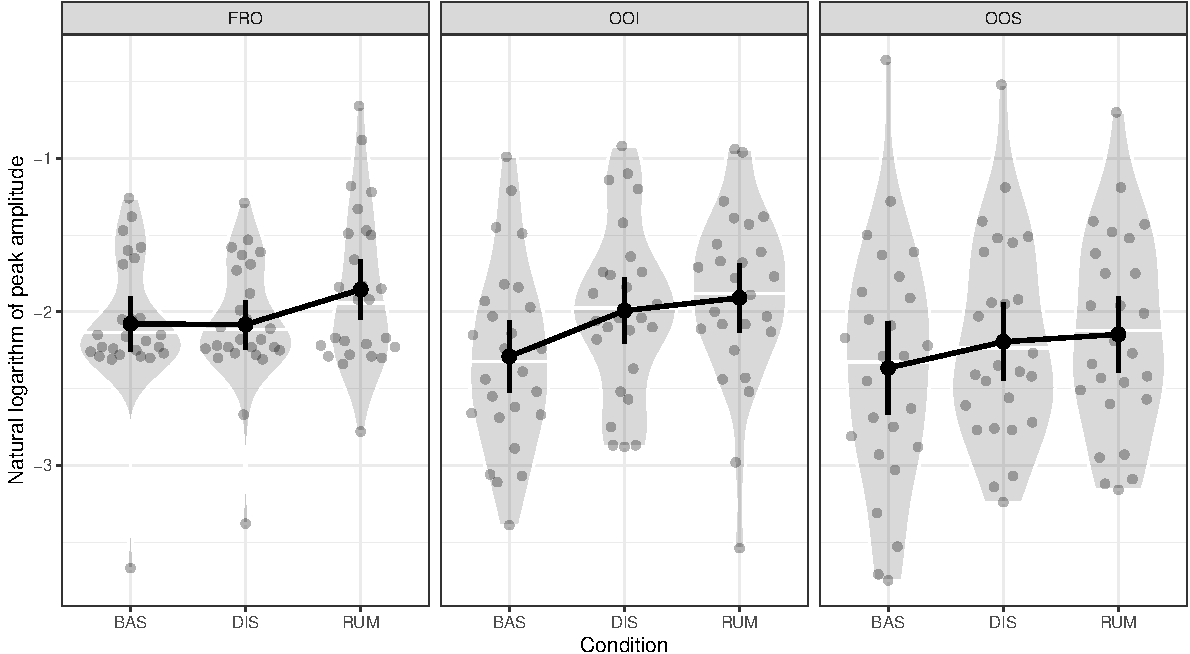
\includegraphics[width=1\linewidth]{reanalysis_files/figure-latex/general-1} 

}

\caption{Average log-EMG amplitude by muscle and condition. The black dots and intervals represent the by-group average and 95\% confidence interval (N = 26). The horizontal white line in the violin plot represents the median. The grey dots represent the individual-level average natural logarithm of the EMG amplitude by muscle and condition.}\label{fig:general}
\end{figure}

\ldots{}

\hypertarget{concluding-on-the-null-from-low-powered-studies}{%
\subsection{Concluding on the null from low-powered studies}\label{concluding-on-the-null-from-low-powered-studies}}

\url{https://theethicalskeptic.com/2015/08/17/the-four-types-of-null-hypothesis-fallacy/}\ldots{}

\ldots{}

\begin{quote}
``In order to test this, a Bayesian paired samples t-test was conducted for the peak log values of muscle activity between the rumination and distraction conditions. This revealed strong evidence in favour of the alternative hypothesis for the FRO muscle (B10 = 18.79), and moderate evidence in favour of the null hypothesis for the OOS (B10 = 0.232) and OOI (B10 = 0.278) muscles, according to current guidelines for interpreting Bayes factors {[}43{]}.''
\end{quote}

Unfortunately, the same line of reasoning applies for testing the effect of the order, which is even less powered than the test of the main effect of interest, rendering it practically uninformative\ldots{}

\begin{figure}[!htb]

{\centering 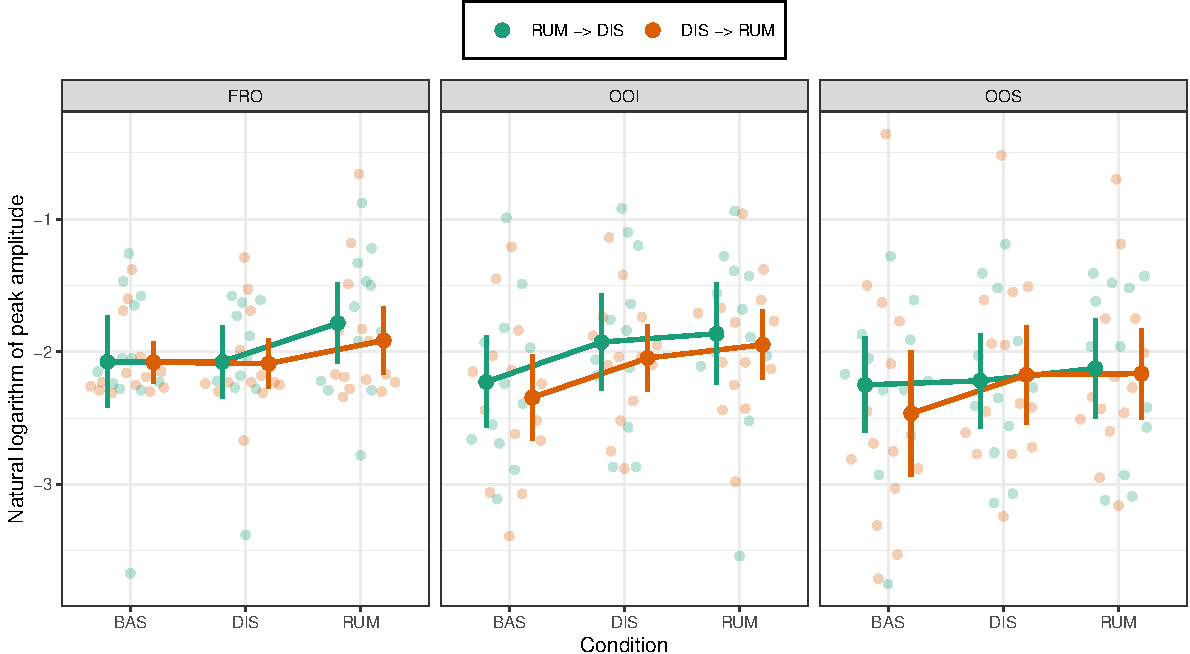
\includegraphics[width=1\linewidth]{reanalysis_files/figure-latex/order-1} 

}

\caption{Average log-EMG amplitude by muscle and condition. The black dots and intervals represent the by-group average and 95\% confidence interval (N = 26). The horizontal white line in the violin plot represents the median. The grey dots represent the individual-level average natural logarithm of the EMG amplitude by muscle and condition.}\label{fig:order}
\end{figure}

\ldots{}

\hypertarget{does-everyone}{%
\subsection{Does everyone?}\label{does-everyone}}

Haaf and Rouder (\protect\hyperlink{ref-haaf_developing_2017}{2017})\ldots{}

\begin{figure}[!htb]

{\centering 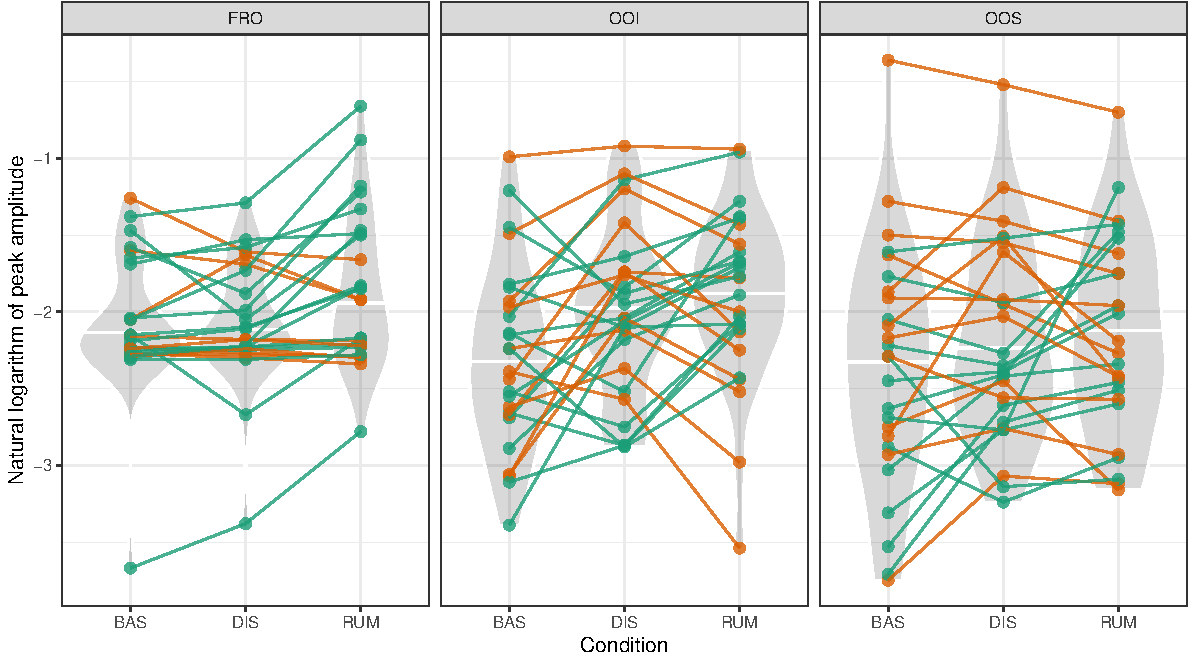
\includegraphics[width=1\linewidth]{reanalysis_files/figure-latex/everyone-1} 

}

\caption{Inter-individual variability in the main effect of interest (i.e., the difference between the rumination and distraction conditions). Green dots and lines represent the average logarithm of the EMG amplitude of participants that showed a higher EMG amplitude in the rumination condition than in the distraction condition, whereas orange dots and lines represent the average logarithm of the EMG amplitude of participants that showed a higher EMG amplitude in the distraction condition than in the rumination condition.}\label{fig:everyone}
\end{figure}

Huge inter-individual variability\ldots{} which leads to the next point, what is the relation between self-reports and EMG?

\hypertarget{relation-between-self-report-and-emg-correlates}{%
\subsection{Relation between self-report and EMG correlates}\label{relation-between-self-report-and-emg-correlates}}

\ldots{}

\hypertarget{discussion-and-conclusions}{%
\section{Discussion and conclusions}\label{discussion-and-conclusions}}

\ldots{}

\hypertarget{supp}{%
\section{Supplementary materials}\label{supp}}

Reproducible code and figures are available at \url{https://github.com/lnalborczyk/inner_experience_EMG}.

\hypertarget{acknowledgements}{%
\section*{Acknowledgements}\label{acknowledgements}}
\addcontentsline{toc}{section}{Acknowledgements}

\ldots{}

\hypertarget{references}{%
\section*{References}\label{references}}
\addcontentsline{toc}{section}{References}

\hypertarget{refs}{}
\begin{cslreferences}
\leavevmode\hypertarget{ref-alderson-day_inner_2015}{}%
Alderson-Day, B., \& Fernyhough, C. (2015). Inner speech: Development, cognitive functions, phenomenology, and neurobiology. \emph{Psychological Bulletin}, \emph{141}(5), 931--965. \url{https://doi.org/10.1037/bul0000021}

\leavevmode\hypertarget{ref-R-papaja}{}%
Aust, F., \& Barth, M. (2017). \emph{papaja: Create APA manuscripts with R Markdown}. \url{https://github.com/crsh/papaja}

\leavevmode\hypertarget{ref-grandchamp_condialint_2019}{}%
Grandchamp, R., Rapin, L., Perrone-Bertolotti, M., Pichat, C., Haldin, C., Cousin, E., Lachaux, J.-P., Dohen, M., Perrier, P., Garnier, M., Baciu, M., \& Lœvenbruck, H. (2019). The ConDialInt Model: Condensation, Dialogality, and Intentionality Dimensions of Inner Speech Within a Hierarchical Predictive Control Framework. \emph{Frontiers in Psychology}, \emph{10}. \url{https://doi.org/10.3389/fpsyg.2019.02019}

\leavevmode\hypertarget{ref-haaf_developing_2017}{}%
Haaf, J. M., \& Rouder, J. N. (2017). Developing constraint in Bayesian mixed models. \emph{Psychological Methods}, \emph{22}(4), 779--798. \url{https://doi.org/10.1037/met0000156}

\leavevmode\hypertarget{ref-loevenbruck_cognitive_2018}{}%
Lœvenbruck, H., Grandchamp, R., Rapin, L., Nalborczyk, L., Dohen, M., Perrier, P., Baciu, M., \& Perrone-Bertolotti, M. (2018). A cognitive neuroscience view of inner language: To predict and to hear, see, feel. In P. Langland-Hassan \& A. Vicente (Eds.), \emph{Inner speech: New voices} (p. 37). Oxford University Press.

\leavevmode\hypertarget{ref-R-wordcountaddin}{}%
Marwick, B. (2019). \emph{Wordcountaddin: Word counts and readability statistics in r markdown documents}.

\leavevmode\hypertarget{ref-moffatt_inner_2020}{}%
Moffatt, J., Mitrenga, K. J., Alderson-Day, B., Moseley, P., \& Fernyhough, C. (2020). Inner experience differs in rumination and distraction without a change in electromyographical correlates of inner speech. \emph{PLOS ONE}, \emph{15}(9), e0238920. \url{https://doi.org/10.1371/journal.pone.0238920}

\leavevmode\hypertarget{ref-R-here}{}%
Müller, K. (2017). \emph{Here: A simpler way to find your files}. \url{https://CRAN.R-project.org/package=here}

\leavevmode\hypertarget{ref-nalborczyk_understanding_2019}{}%
Nalborczyk, L. (2019). \emph{Understanding rumination as a form of inner speech: Probing the role of motor processes} {[}PhD Thesis{]}. Univ. Grenoble Alpes \& Ghent University.

\leavevmode\hypertarget{ref-nalborczyk_introduction_2019}{}%
Nalborczyk, L., Batailler, C., Lœvenbruck, H., Vilain, A., \& Bürkner, P.-C. (2019). An introduction to Bayesian multilevel models using brms: A case study of gender effects on vowel variability in standard indonesian. \emph{Journal of Speech Language and Hearing Research}, \emph{62}(5), 1225--1242. \url{https://doi.org/10.1044/2018_JSLHR-S-18-0006}

\leavevmode\hypertarget{ref-nalborczyk_can_2020}{}%
Nalborczyk, L., Grandchamp, R., Koster, E. H. W., Perrone-Bertolotti, M., \& Lœvenbruck, H. (2020). Can we decode phonetic features in inner speech using surface electromyography? \emph{PLOS ONE}, \emph{15}(5), e0233282. \url{https://doi.org/10.1371/journal.pone.0233282}

\leavevmode\hypertarget{ref-nalborczyk_orofacial_2017}{}%
Nalborczyk, L., Perrone-Bertolotti, M., Baeyens, C., Grandchamp, R., Polosan, M., Spinelli, E., Koster, E. H. W., \& Lœvenbruck, H. (2017). Orofacial electromyographic correlates of induced verbal rumination. \emph{Biological Psychology}, \emph{127}, 53--63. \url{https://doi.org/10.1016/j.biopsycho.2017.04.013}

\leavevmode\hypertarget{ref-perrone-bertolotti_what_2014}{}%
Perrone-Bertolotti, M., Rapin, L., Lachaux, J. P., Baciu, M., \& Lœvenbruck, H. (2014). What is that little voice inside my head? Inner speech phenomenology, its role in cognitive performance, and its relation to self-monitoring. \emph{Behavioural Brain Research}, \emph{261}, 220--239. \url{https://doi.org/10.1016/j.bbr.2013.12.034}

\leavevmode\hypertarget{ref-R-base}{}%
R Core Team. (2017). \emph{R: A language and environment for statistical computing}. R Foundation for Statistical Computing. \url{https://www.R-project.org/}

\leavevmode\hypertarget{ref-R-tidyverse}{}%
Wickham, H. (2017). \emph{Tidyverse: Easily install and load the 'tidyverse'}. \url{https://CRAN.R-project.org/package=tidyverse}

\leavevmode\hypertarget{ref-wilkinson_auditory_2017}{}%
Wilkinson, S., \& Fernyhough, C. (2017). Auditory verbal hallucinations and inner speech: A predictive processing perspective. In Z. Radman (Ed.), \emph{Before Consciousness: In Search of the Fundamentals of Mind}. Imprint Academic, Ltd.

\leavevmode\hypertarget{ref-R-knitr}{}%
Xie, Y. (2015). \emph{Dynamic documents with R and knitr} (2nd ed.). Chapman; Hall/CRC. \url{https://yihui.org/knitr/}

\leavevmode\hypertarget{ref-R-rmarkdown}{}%
Xie, Y., Allaire, J. J., \& Grolemund, G. (2018). \emph{R markdown: The definitive guide}. Chapman; Hall/CRC. \url{https://bookdown.org/yihui/rmarkdown}
\end{cslreferences}

\end{document}
